\documentclass[runningheads,a4paper]{llncs}

\usepackage[cmex10]{amsmath}
\usepackage{graphicx}
\usepackage{booktabs}
\usepackage{tabularx}
\usepackage{rotating} 
\usepackage{color}
\usepackage{subfig}
\usepackage[unicode,
					  colorlinks,
						linkcolor={red},
						citecolor={blue},
						urlcolor={blue},
            pdfauthor={Arkadiusz Jachnik, Maciej Piernik},
            pdftitle={State--changing sequential pattern mining using uplift modeling},
            pdfsubject={Sequential pattern mining},
            pdfkeywords={sequential patterns, uplift modeling}]{hyperref}

\newcolumntype{R}{>{\raggedleft\arraybackslash}X}
\newcommand{\argmax}[1]{\underset{#1}{\operatorname{argmax}}\;}
\newcommand{\matr}[1]{\mathbf{#1}}

\begin{document}

\mainmatter

\title{State--changing sequential patterns}

\titlerunning{State--changing sequential patterns}

\author{Arkadiusz Jachnik \and Maciej Piernik}

\authorrunning{Arkadiusz Jachnik \and Maciej Piernik}

\institute{Institute of Computing Science, Poznan University of Technology\\
ul. Piotrowo 2, 60--965 Poznan, Poland\\
\email{maciej.piernik@cs.put.poznan.pl}}

\maketitle

\begin{abstract}
Designing algorithms for finding more meaningful patterns is one of the most important challenges in the field of sequential pattern mining.
Additional data, when properly incorporated into the analysis, may help tailor the solution to the specific business requirement.
Such a situation takes place in sequences of events targeted at certain objects (e.g., marketing campaigns, medical treatment, etc.) when state of the objects is being additionally monitored (e.g., client's attitude towards a brand or patient's health).
In this paper, we propose to combine the information about the events with the information about state in mining for sequential patterns of events.
Our solution is designed to allow for a more meaningful assessment of the influence of a given sequence of events on a given direction of change of an object's state (up, down, or no change).
To be able to properly interpret the changes in states as outcomes of sequences of events, we rely on the concept of a control group and uplift modeling.
The state--changing sequential patterns are created in a three--step process involving sequential pattern mining, mapping states to changes, and calculating the uplift of each pattern.
To illustrate the usefulness of our proposal in practical scenarios, we perform an experiment on 3 real--world datasets.
Furthermore, we compare the outcomes of the uplift measure with 10 other measures used to assess the quality of sequential patterns.
The results reveal that our method allows to find sequences which could otherwise be neglected.
\keywords{sequential patterns, uplift modeling}
\end{abstract}

\section{Introduction}
\label{sec:introduction}

Sequential patterns are an extension of frequent patterns (or frequent itemsets, known from association rule mining) to sequential data.
They find many applications in domains such as customer transaction analysis, web mining, software bug analysis, chemical and biological analysis~\cite{Aggarwal:2014}.
Just like with traditional frequent patterns, there are many versions of sequential patterns, depending on the structure of the sequences.
For instance, each event in a sequence can be either a single item or an itemset; precedence of elements can be implied solely by their order or explicitly by time; time can be used to further narrow the problem by constraining time gaps between elements; each event in a sequence can be described by a symbol, a number, or a set of features, etc.~\cite{Dong:2009}.
On top of that, in scenarios such as classification, class information can be added to each element in each sequence.
This results in a setting where a dataset contains sequences of pairs $\langle\texttt{event}, \texttt{class}\rangle$.
In many real-world scenarios, however, such a setting is impossible to achieve, as the class information may be provided with a delay or even completely asynchronously from the analyzed events.
Consider a sequence of treatments prescribed to a given patient for a certain disease measured by some indicator (e.g., blood pressure).
After a series of events (e.g., administered pharmaceuticals, medical procedures, dietary regulations) the indicator may either improve, worsen, or stay unchanged.
However, this result does not necessarily coincide with any of the events nor need it be a result of one, all, or any of the events.
This scenario is universal when modeling people's behavior, opinion, or --- more generally speaking --- \textit{state}.
As illustrated by the examples above, this problem is no longer described by a single sequence of events (like in classical sequential pattern mining), but rather by two connected sequences --- one with the events and the other with classes.
To the best of our knowledge, processing of sequential data of such composition has not yet been considered and is the focus of this research.

The assumption underlying the described scenario is that the events in the sequences influence the outcomes registered by the classes.
A classical example of such an analysis performed on traditional data is the aforementioned clinical trial.
In order to properly model the outcomes of patients' treatments, the results need to be evaluated against a control group.
A method aiming specifically at this task is uplift modeling, as it's goal, as originally formulated, is to model the change in peoples' behavior as a result of intentional activity~\cite{Radcliffe:1999}.

In this paper, we propose a solution to the problem of finding state--changing sequential patterns.
Our method is designed to work in a setting where the information about states (classes) is provided separately from the underlying sequence of events.
Inspired by clinical trials, it relies on the notion of a control group and uses uplift modeling to factor this notion into the processing.
We experimentally evaluate our proposal using real-world data to showcase its applicability in practical situations.

The remainder of this paper is organized as follows.
Section~\ref{sec:related} outlines the research related to our proposal.
In Section~\ref{sec:main}, we formally define state--changing sequential patterns and show how to find them.
In Section~\ref{sec:experiments}, we experimentally evaluate our proposal and discuss the obtained results.
Finally, in Section~\ref{sec:conclusions}, we conclude the paper and draw lines of future research.

\section{Related Work}
\label{sec:related}
As more and more data generated every day come in the form of sequences, mining in sequential data has been extensively studied over the recent decades~\cite{Dong:2009,Fournier:2017}.
Sequential pattern mining is probably the most studied field in this area and many algorithms have been proposed to solve this problem.
One of the first attempts at addressing this problem was an extension of a well known pattern mining algorithm Apriori~\cite{Agrawal:1994}, called AprioriAll~\cite{Agrawal:1995}.
Although straightforward, the algorithm suffers from low efficiency due to multiple database scans and generating massive candidate sets.
As a natural consequence, many other approaches followed, aiming at reducing the complexity of the mining process, examples of which are Spade~\cite{Zaki:2001}, PrefixSpan~\cite{Pei:2004}, Lapin~\cite{Yang:2007}, or CM-Spade~\cite{Fournier:2014}.

Several methods were also introduced to mine for sequential patterns with additional constraints, most notably, closed and maximal sequential patterns as well as sequential patterns with time constraints.
Closed sequential patterns, apart from being frequent, have an additional restriction of not having any supersequence with the same frequency in the dataset among other patterns.
This can drastically reduce the number of generated patterns, yet, it is still possible to recover all sequential patterns along with their support without the necessity to scan the dataset.
Examples of algorithms mining for such patterns are CloSpan~\cite{Yan:2003} and BIDE~\cite{Wang:2004}.
Maximal sequential patterns restrict the patterns even further, so that no pattern can have any supersequence among other patterns.
This reduces the number of patterns even further, however, this process is not fully reversible.
After applying the restriction, other sequential patterns can be recreated, however, without the information about their support (only the lower--bound is known from the maximal patterns).
Examples of algorithms dedicated to finding maximal sequential patterns are MaxSP~\cite{Fournier:2013} and VMSP~\cite{Fournier:2014-2}.
The most well--known method for finding time--constrained sequential patterns is GSP~\cite{Srikant:1996}.
As it's most notable feature, GSP puts time restrictions on the gaps between elements appearing in a pattern, so that two elements cannot appear too close or too far after one another.

All of these approaches can be used to tackle the problem defined in this paper, i.e., to find frequent patterns of events.
However, as they are all dedicated for general, single--sequence problems, they are unable to include the information about how these patterns would affect the objects' states.
To the best of our knowledge, our proposal is the first attempt at solving this problem.
As our method performs sequential pattern mining in the first step, it could in principle use any of the above--defined methods.
Therefore, the research stated in this paper is different from the previous methods, yet, complementary.

In the context of assessing the usefulness of a given pattern, many methods have been proposed for non--sequential data in the context of association rule mining~\cite{Lenca:2007,Tan:2002}.
However, we did not find any measures which would be sequential--data--specific, let alone designed for sequences of events with state.
As our goal is to measure the influence a given sequential pattern has on a particular direction of change in state, we rely on a measure inspired by uplift modeling~\cite{Radcliffe:1999}.
However, our experiments show that other measures of effect, like relative risk, could be used with the same result.

\section{State--changing sequential patterns}
\label{sec:main}

\subsection{Conceptual description}
To illustrate both, the problem we are tackling and our proposed solution, consider the following example.
Assume we have a history of marketing campaigns conducted by some company to it's clients.
The history of campaigns directed at a single client (in order of their occurrence) forms a single sequence of events.
Furthermore, assume that, from time to time, the company also monitored it's clients opinion about the company.
The opinion can be either negative, neutral, or positive (where negative $<$ neutral $<$ positive).
The history of a single client's opinions (in order of the time they were queried) forms a single sequence of the client's states.
Both of these sequences form a complete client's history, example of which is illustrated in Fig.~\ref{fig:example}.

\begin{figure}[!ht]
	\centering
		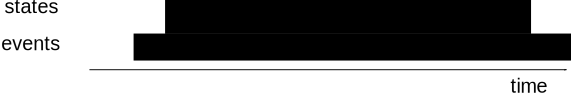
\includegraphics[width=0.75\textwidth]{images/example}
	\caption{Example of an analyzed sequence, where each $e_i$ represents events for a given object (e.g., marketing campaigns directed at a given client) and each $s_i$ represents the object's states (e.g., negative, neutral, or positive opinion about a given brand).}
	\label{fig:example}
\end{figure}

Given the above, the problem of state--changing sequential patterns can be formulated as follows.
Is it possible to find a subsequence of events (e.g., marketing campaigns) which will have a high probability of influencing the objects' state in a desired manner (e.g., improving the clients' opinion about a brand).

Our proposed solution for the above--defined problem is a 3-step generic method, which can be described as follows.
In the first step, we mine the sequences of events for frequent sequential patterns, i.e., subsequences, which appear in the events dataset with a required minimal frequency.
In the second step, we map the states sequences to sequences of directions of change.
Each state is mapped to a change indicator based on it's relation to the previous state.
A change from a lower to a higher state is encoded as ``$\uparrow$'' (\textit{up}); a change from a higher to a lower state is encoded as ``$\downarrow$'' (\textit{down}); and no change is encoded as ``$\emptyset$'' (\textit{none}).
The first state is mapped to ``$\emptyset$''.
In the third phase, we calculate the uplift measure of each sequential pattern for a given change indicator (e.g., ``$\uparrow$''), by contrasting the probability of this change appearing after a given pattern among the sequences with this pattern against the probability of this change appearing among the sequences without this pattern.
After this process, we have a list of sequential patterns with the information about their impact on a given change of state.
The whole process is summarized in Fig.~\ref{fig:concept}.

\begin{figure}[!ht]
	\centering
		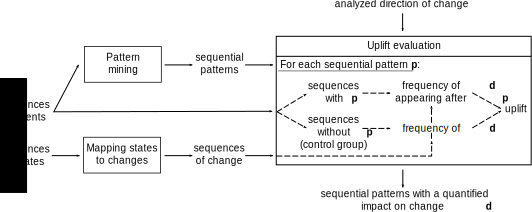
\includegraphics[width=\textwidth]{images/concept}
	\caption{Illustration of the proposed method}
	\label{fig:concept}
\end{figure}

\subsection{Formal description}
By a \textit{sequence} $s=\textless s_1, s_2, ..., s_n\textgreater$ we understand an ordered multi--set of \textit{elements}, where each element $s_i$ is drawn from the same set.
We distinguish two sets of sequences: sequences of events $\mathcal{S}^e$ and sequences of states $\mathcal{S}^s$, where the elements in the events sequences are drawn from the events set and the elements in the states sequences are drawn from the ordered states set.
Each events sequence $s^e\in\mathcal{S}^e$ has a corresponding states sequence $s^{se}\in\mathcal{S}^s$ (note that this correspondence is only one--sided).
The corresponding sequences can be combined into a single sequence of events and states and there exists a total order between the elements of the combined sequences such that the order of the elements from each sequence is preserved.

A sequence $s'$ which elements form a subset of elements of another sequence $s$ is called a \textit{subsequence} of $s$ and is denoted as $s'\subseteq s$.
Given a set of sequences $\mathcal{S}$, a sequence $p$ is called a \textit{sequential pattern} (or \textit{pattern}), if it is a subsequence of at least \textit{minsup} sequences in $\mathcal{S}$: $|\{s\in\mathcal{S}:p\subseteq s\}|\geq\textit{minsup}$, where \textit{minsup} is a user--defined minimal support parameter.
We denote that a sequence $s$ \textit{contains} a pattern $p$ if $p\subseteq s$.
Given a sequence $s=\textless s_1,s_2,...,s_n\textgreater$, its subsequence $s'=\textless s_{i_1}, s_{i2}, ..., s_{i_m}\textgreater$, $1\leq m\leq n$, and an element $s_x\in s$, we say that $s_x$ appears in $s$ after $s'$ if $i_m<x\leq n$.

Given the above, our method is defined as follows.
Given a set of event sequences $\mathcal{S}^e$, a set of state sequences $\mathcal{S}^s$, a desired direction of change \textit{d}, and a minimal support threshold \textit{minsup}, first, we are mining $\mathcal{S}^e$ for sequential patterns $\mathcal{P}=\left\{p:|\{s^e\in\mathcal{S}^e:p\subseteq s^e\}|\geq\textit{minsup}\right\}$.
Next, each sequence of states $s^s\in\mathcal{S}^s$ is mapped into a sequence of changes $s^c\in\mathcal{S}^c$:
\begin{equation*}
\begin{split}
&s^c_1=-\\
&s^c_i=\begin{cases}
	\uparrow & s^s_{i-1}<s^s_i \\
	\downarrow & s^s_{i-1}>s^s_i \\
	\emptyset & otherwise
\end{cases}
\end{split}
\end{equation*}
where $i=2..|s^s|$.
The mapping preserves the correspondence relation with the events sequence and the total order of the combined elements of the events and changes sequences.
Finally, for each sequential pattern $p\in\mathcal{P}$ and a given change direction $d$, \textit{uplift} is calculated according to the following formula:
\begin{equation*}
\textit{uplift}(p,d)=P(d^p|\{s^e\in\mathcal{S}^e:p\subseteq s^e\})-P(d|\{s^e\in\mathcal{S}^e:p\not\subseteq s^e\}),
\end{equation*}
where $P(d^p|\{s^e\in\mathcal{S}^e:p\subseteq s^e\})$ denotes the probability of $d$ appearing after $p$ in sequences of events containing $p$, and $P(d|\{s^e\in\mathcal{S}^e:p\not\subseteq s^e\})$ denotes the probability of $d$ appearing in sequences of events without $p$.

\section{Experiments}
\label{sec:experiments}
\subsection{Experimental Setup}
This paper intends to evaluate the possibility of using state--changing sequential patterns as a means to analyzing real--world datasets as well as to assess the rightness of choice of uplift modeling to measure the influence of sequential patterns of events on a given direction of change in state.
Our solution was evaluated in a series of experiments using anonymized private data and publicly available datasets.
We processed full datasets with different support values for each of them using the Apriori algorithm to find sequential patterns.
Furthermore, we calculated several measures for evaluating the quality of patterns, such as support, confidence, coverage, prevalence, recall, lift, leverage, added value, Jaccard, and relative risk, to assess the extent of influence of each pattern on the ``$\uparrow$'' direction of change.
Afterward, we compared these measures with the uplift measure and analyzed the results. 

The experiments were prepared using software components implemented in R language.
Almost all of the software components were implemented using R standard library.
The exception is the component used for generating two--element permutations of sequential candidate patterns, where we used ``gtools'' library.
The experiments were conducted on a machine equipped with a quad-core I7-4770HQ @ 2,2 GHz processor and 16 GB of RAM.

\subsection{Datasets}
To prepare the experimental evaluation of the proposed solution, we used three datasets containing sequential data.
The \textit{diabetes} dataset is publicly available through the UCI Machine Learning Repository~\cite{Kahn:1994}.
It includes data about the activity of diabetes people and blood sugar level measurements.
A private marketing company provided the \textit{events} dataset.
It contains data about marketing activity as well as the outcome of this activity.
The \textit{fifa} dataset contains data about clickstream from the FIFA World Cup 98 webpage.
It is publicly available on the website of SPMF – an open source data mining library~\cite{Fournier}.
Table \ref{tab:datasets} presents the summary of each dataset.

To test the proposed solution, we had to augment two of the datasets with the information about states, which was not explicitly distinguished in the data.
The \textit{diabetes} dataset contains numeric attribute describing blood sugar level.
We discretized this attribute into three states describing blood sugar level as high, normal, and low, respectively.
Regarding the \textit{fifa} dataset, we generated the missing sequences of states based on the original data.
To each event, we assigned one of the three values describing the length of a subsequence, denoted as short, medium and long.
A subsequence starts with the first element of the original sequence and finishes with a given event occurrence.

\begin{table}[htbp]
	\scriptsize
  \centering
  \caption{Characteristics of datasets}
    \begin{tabularx}{\textwidth}{l@{}R@{}R@{}R@{}R@{}R@{}R@{}}
		\toprule
	{} & \multicolumn{3}{c}{Sequence of events} & \multicolumn{3}{c}{Sequence of states} \\
        \toprule
    Dataset & \#Instances & \#Elements & Avg. len. & \#Instances & \#Elements & Avg. len.\\
		\midrule
	\textit{diabetes}              &	3883	    &    20    &    7.6    &    3883    &    3    &    7.6 \\
		\midrule
	\textit{events} &	4656	    &    114   &	   21.2   &    10685   &    3    &    26,5 \\
		\midrule
	\textit{fifa}	                  &  20450    &  	29990  &   34.74   &    29990  &     3    &    34.74 \\
        \bottomrule
    \end{tabularx}%
  \label{tab:datasets}%
\end{table}%

\subsection{Results}
Table~\ref{tab:results} presents the results of our experiments.
It contains five sequential patterns with the highest uplift measure from each of the datasets.
We juxtaposed these results with the other pattern evaluation measures described above.
Values marked in bold represent the best result of a given measure for a particular dataset.

We processed the \textit{diabetes} dataset with $\textit{minsup} = 0.4$, and, as a result, we found 89 sequential patterns.
The values of uplift measure for these sequential patterns were from the range $[-0.28, 0.21]$.
Pattern $\textless 58\textgreater$ was found to have the highest value of uplift measure.
The event 58 corresponds to pre--breakfast blood glucose measurement, so it is the first activity which diabetes people do every day and also the one about which is the most difficult to forget during a daily run, what is confirmed in the high support value of this sequential pattern.
Because during the day fluctuations of the blood sugar level could be high, it is also highly possible that we will notice a decrease in blood sugar level, what is illustrated by the high confidence level.

Regarding the \textit{events} dataset, we processed this dataset with $\textit{minsup} = 0.45$.
We found 12 sequential patterns.
The values of the uplift measure were from the range $[0.14, 0.25]$.
Pattern $\textless 34, 109\textgreater$ has the highest uplift value.
We do not have information about which marketing activity these two events describe, but the value of uplift measure suggests that these consecutive activities positively influence customers’ attitude towards the brand.
The support value points out that this pattern is included in around 47\% of all sequences, while the confidence value shows that occurrence of this pattern positively affected customers in 40\%.

Finally, we found 5 sequential patterns with $\textit{minsup}=0.4$ in the \textit{fifa} dataset.
The values of uplift measure were from the range $[0.38, 0.43]$.
The highest value of uplift measure can be found in pattern $\textless 90\textgreater$.
We do not have the information about which website is described by the $90$ event in the dataset, but high value of the uplift measure indicates that users stayed longer on the FIFA website after seeing the content of this website.
The support and confidence values were respectively 0.40 and 0.97.

We noticed the high correlation between uplift and relative risk measures for each of the analyzed dataset.
To understand why this correlation exists, it is required to take a closer look at the structure of these measures.
Uplift tries to estimate the increase of some event's occurrence probability in a treated subpopulation over the corresponding probability when the subpopulation was not treated, whereas relative risk is the ratio of the same probabilities.
Thus, uplift presents the actual change of probability, while relative risk expresses the relative relation between probabilities.

Other measures evaluated during our experiments performed with a varying result.
To understand this fact, it is again required to analyze the differences between the construction of uplift measure and other measures used in this experiment.
Uplift divides the probability space into treated and not treated subspaces, while measures like coverage, prevalence, recall, lift, leverage, added value, and Jaccard estimate the probability of event occurrence by considering the entire probability space.
This fact may lead to wrong interpretation of the obtained results and, in consequence, to wrong and potentially costly mistakes in decision--making based on this interpretation.

\begin{sidewaystable}[htbp]
	\scriptsize
  \centering
  \caption{Results of the experimental evaluation}
    \begin{tabularx}{\textwidth}{l@{}c@{}R@{}R@{}R@{}R@{}R@{}R@{}R@{}R@{}R@{}R@{}R@{}R@{}}
		\toprule
	{} & \multicolumn{2}{c}{Sequential pattern} & \multicolumn{11}{c}{Pattern quality measures} \\
        \toprule
    Dataset          & Seq. pattern                                                                                      & Support & Class order & Uplift      & Support   & Confidence & Coverage  & Recall    & Lift      & Leverage  & Added value & Jaccard   & Relative risk\\
		\midrule
	\textit{diabetes}         & $\textless 58\textgreater$                                                         & \textbf{0.90}                  & h \textless n \textless l   & \textbf{0.21} & \textbf{0.88} & 0.98 & \textbf{0.90}  & \textbf{0.92} & 1.02 & 0.11 & 0.02 & \textbf{0.90} & \textbf{1.28} \\
		\midrule                             
	\textit{diabetes}         & $\textless 58,33\textgreater$                              & 0.80                  & h \textless n \textless l   & 0.13 & 0.79 & 0.99 & 0.80  & 0.82 & 1.03 & 0.22 & 0.02 & 0.81 & 1.14 \\
		\midrule                             
	\textit{diabetes}         & $\textless 58,33,33\textgreater$   & 0.73                  & h \textless n \textless l   & 0.09 & 0.73 & 0.99 & 0.73  & 0.75 & 1.03 & 0.28 & 0.02 & 0.75 & 1.10 \\
		\midrule                             
	\textit{diabetes}         & $\textless 33\textgreater$  & 0.87 & h \textless n \textless l & 0.09 & 0.85 & 0.98 & 0.87 & 0.88 & 1.01 & 0.14 & 0.01 & 0.86 & 1.10 \\
		\midrule                             
	\textit{diabetes}         & $\textless 58,62,33\textgreater$ & 0.68 & h \textless n \textless l & 0.08 & 0.67 & \textbf{0.99} & 0.68 & 0.69 & \textbf{1.03} & \textbf{0.34} & \textbf{0.03} & 0.69 & 1.09 \\
	    \midrule
	    \midrule
    \textit{events}   & $\textless 34,109\textgreater$ & 0.46 & a \textless b \textless c & \textbf{0.25} & \textbf{0.19} & \textbf{0.40} & 0.46 & \textbf{0.70} & \textbf{1.50} & 0.28 & \textbf{0.13} & \textbf{0.34} & \textbf{2.68} \\
        \midrule
    \textit{events}   & $\textless 109\textgreater$ & \textbf{0.47} & a \textless b \textless c & 0.25 & \textbf{0.19} & 0.40 & \textbf{0.47} & 0.70 & 1.50 & 0.28 & 0.13 & 0.34 & 2.68 \\
        \midrule
    \textit{events}   & $\textless 108,34\textgreater$ & 0.45 & a \textless b \textless c & 0.24 & 0.18 & 0.40 & 0.45 & 0.68 & 1.50 & \textbf{0.28} & 0.13 & 0.34 & 2.56 \\
        \midrule
    \textit{events}   & $\textless 108\textgreater$  & 0.45 & a \textless b \textless c & 0.24 & 0.18 & 0.40 & 0.45 & 0.68 & 1.50 & 0.28 & 0.13 & 0.34 & 2.55 \\
        \midrule
    \textit{events}   & $\textless 108,34,109\textgreater$ & 0.45 & a \textless b \textless c & 0.24 & 0.18 & 0.40 & 0.45 & 0.68 & 1.49 & 0.28 & 0.13 & 0.34 & 2.55 \\
	    \midrule
	    \midrule
	\textit{fifa} & $\textless 90\textgreater$ & 0.40 & s \textless m \textless l & \textbf{0.43} & 0.39 & \textbf{0.98} & 0.40 & 0.55 & \textbf{1.36} & \textbf{0.69} & \textbf{0.26} & 0.54 & \textbf{1.80} \\
	    \midrule
    	\textit{fifa} & $\textless 13\textgreater$ & 0.40 & s \textless m \textless l & 0.43 & 0.39 & 0.97 & 0.40 & 0.54 & 1.36 & 0.68 & 0.26 & 0.26 & 1.78 \\
    	    \midrule
    \textit{fifa} & $\textless 18\textgreater$ & 0.40 & s \textless m \textless l & 0.42 & 0.39 & 0.96 & 0.40 & 0.54 & 1.35 & 0.67 & 0.25 & 0.53 & 1.76 \\
        \midrule
    \textit{fifa} & $\textless 30\textgreater$ & \textbf{0.42} & s \textless m \textless l & 0.39 & \textbf{0.40} & 0.94 & \textbf{0.43} & \textbf{0.56} & 1.31 & 0.63 & 0.22 & \textbf{0.54} & 1.72 \\
        \midrule
    \textit{fifa} & $\textless 2\textgreater$ & 0.40 & s \textless m \textless l & 0.38 & 0.38 & 0.95 & 0.40 & 0.52 & 1.32 & 0.66 & 0.23 & 0.51 & 1.68 \\
        \bottomrule
    \end{tabularx}%
  \label{tab:results}%
\end{sidewaystable}%


\section{Conclusions}
\label{sec:conclusions}
In this paper, we presented a solution to the problem of finding subsequences of events (e.g., marketing campaigns) with high probability of influencing the state of the objects targeted by these events (e.g., changing the clients’ opinion about a given brand).
We call such subsequences state--changing sequential patterns.
Our method works by mining for frequent patterns in the events sequences, mapping the states sequences to sequences encoding the changes in state, and evaluating the influence of the obtained patterns on these changes using uplift modeling.
The intuition behind our solution was to take the approach common from clinical trials and extend it to sequential data.
By experimentally testing our proposal on 3 real--world datasets we validate its usefulness for practical problems.
Furthermore, we empirically compare the employed uplift measure with 10 other measures used for sequential pattern evaluation.
The results reveal that our method allows to find sequences which could otherwise be neglected.
It also shows that uplift could be used interchangeably with relative risk, however, this was to be expected as these measures belong to the same family and are highly related.

As the issue tackled in this paper is itself novel, the possibilities of extending this work are very broad.
As our most immediate future research focus, we plan on experimenting with introducing time constraints to the problem.
The constraints could concern both, events (e.g., restricting time gaps between events) and states (e.g., the certainty of a given object's state can decay over time until new state appears).
Moreover, we intend to create other sequential pattern evaluation measures dedicated for this specific problem.
We would also like to quantify the differences between states and include those differences in the analysis, as our current approach only registers the changes in states' direction.

\subsubsection*{Acknowledgments.} This research is partly funded by the Polish National Science Center under Grant No. DEC-2015/19/B/ST6/02637.

\bibliographystyle{splncs}
\bibliography{Bibliography}

\end{document}
